\documentclass{article}



\def\subj {MATH}
\def\npart {407}
\def\nterm {Fall}
\def\nyear {2018}
\def\ncourse {Complex Variables}

\input{header}

\begin{document}
\maketitle
{\small
  \noindent\textbf{The Complex Number Plane}\\
  Introduction to complex numbers, the complex plane, point sets in the plane, stereographic projection; the extended complex plane, curves and regions.\hspace*{\fill} [1]

  \vspace{10pt}
  \noindent\textbf{Functions of a Complex Variable}\\
  Functions and limits, differentiability and analyticity, the Cauchy-Riemann conditions, linear fractional transformations, transcendental functions, Riemann surfaces.\hspace*{\fill} [2]

  \vspace{10pt}
  \noindent\textbf{Integration in the Complex Plane}\\
  Line integrals, Cauchy's theorem, Cauchy formulas, Maximum Modulus Principle.\hspace*{\fill} [3]

  \vspace{10pt}
  \noindent\textbf{Sequences and Series}\\
  Sequences of complex numbers; functions, infinite series, power series, analytic continuation, Laurent series, Double series, infinite products, improper integrals, the Gamma function.\hspace*{\fill} [4]

  \vspace{10pt}
  \noindent\textbf{Residue Calculus}\\
  The Residue theorem, evaluation of real integrals, the principle of the argument, meromorphic functions, entire functions.\hspace*{\fill} [5]
  }

\tableofcontents

\setcounter{section}{0}
\section{The Complex Numbers}

	\textbf{Question}: Does $x^2+1=0$ have any solutions?
	\begin{itemize}
		\item No: If we look for real solutions 
		\item Yes: If we have a more general notion of numbers
	\end{itemize}	

	\noindent We introduce $i$ so that $i^2 = -1$.

	\begin{defi}
		$\C$ is the set of complex numbers formed as $z=x+iy$, $x,y \in \R$. The \textit{real part}, $x$, is written as $\Re(z)$, and the \textit{imaginary part}, $y$, is written as $\Im(z)$.
	\end{defi}

	\begin{note}
		We can identify $\C$ with points in $\R^2$ by the correspondence $(x+iy) \leftrightarrow (x,y)$.
	\end{note}

	
	\begin{defi}[Addition/Subtraction]
		We add/subtract complex numbers by their real and imaginary components respectively.
		\[
			(a+ib) \pm (c+id) = (a\pm c) + i(b \pm d)
		\]
	\end{defi}

	\begin{defi}
		The \textit{Modulus} (absolute value) of $z=x+iy$ is the length of the vector $(x,y)$ which is $\sqrt{x^2+y^2}$, and is denoted as $|z|$.
	\end{defi}

	\begin{defi}[Triangle Inequality]

		For vectors, we have the triangle inequality
		\[
			|\vec{u} + \vec{v}| \leq |\vec{u}| + |\vec{v}|
		\]
		For $\C$, this translates to
		\[
			|z_1 + z_2| \leq |z_1| + |z_2|
		\]
		There is also a useful variant: \\
	
			Apply to $z=(z-w) + w$, where $z,w \in \C$.
			\begin{align*}
				|z| &\leq |z-w| + |w| \\
				|z-w| &\geq |z| - |w| \\
				|w| - |z| &\leq |w-z| = |z-w| \\
				\Rightarrow |z-w| &\geq \big| |z| - |w| \big| 
		\end{align*}
	\end{defi}

	\begin{defi}[Multiplication]
		For multiplying two complex numbers, we expand each binomial and collect the real and imaginary parts respectively.
		\[
			(a+ib)(c+id) = (ac-bd) + i(bc + ad)
		\]
	\end{defi}

	The usual algebraic rules still apply for complex numbers.
	\begin{alignat*}{2}
		(z_1 z_2) z_3 &= z_1(z_2 z_3) \qquad  &&\text{associative} \\
		z_1 z_2 &= z_2 z_1 \qquad &&\text{commutative} \\
		z_1(z_2 + z_3) &= z_1 z_2 + z_1 z_3 \qquad &&\text{distributive}
	\end{alignat*}

	\begin{eg}[Proof of commutative] $ $
		\begin{proof}
			\begin{align*}
				(a+ib)(c+id) &= (ac-bd) + i(bc + ad) \\
				(c+id)(a+ib) &= (ca-db) + i(cb + da)
			\end{align*}
		\end{proof}
	\end{eg}

	\begin{defi}[Complex conjugate]
		If $z=x+iy$, then its complex conjugate, denoted as $\bar{z}$, is $\bar{z} = x-iy$.
	\end{defi}

	\begin{eg}
		If we compute $z\bar{z}$, we get
		\begin{align*}
			(z+iy)(z-iy) &= x^2 + y^2 + i(yx-xy) \\
			&= x^2 + y^2 \\
			&= |z|^2
		\end{align*}
		i.e $z\bar{z} = |z|^2$.
	\end{eg}
	Some other useful properties:
	\begin{align*}
		\overline{(z+w)} &= \bar{z} + \bar{w} \\
		\overline{zw} &= \bar{z} \bar{w} \\
		|\bar{z}| &= |z|
	\end{align*}

	\begin{note}
		$z+\bar{z}/2 = x$ , $z-\bar{z}/2i = y$.
	\end{note}

	\begin{defi}[Inverses]
		If $z\neq 0$, then $1/z$ exists as a complex number. We have
		\[
			z\bar{z} = |z^2|
		\]
		or
		\[
			\frac{1}{z} = \frac{\bar{z}}{|z|^2}
		\]
	\end{defi}

	\begin{defi}[Division]
		It follows from the definition of a complex inverse,
		\[
			\frac{z}{w} = \frac{z\bar{w}}{w\bar{w}} = \frac{z\bar{w}}{|w|^2}
		\]
	\end{defi}

	\begin{thm}[Fundamental Theorem of Algebra]
		Every polynomial can be expressed as a product of linear factors \underline{over $\C$}. This is equivalent to the statement that every polynomial equation $p(z)=0$ has a solution.
	\end{thm}

	\begin{proof}
		Suppose a polynomial $p(z)$ factors as $(z-z_{1})(z-z_{2}) \dots (z-z_{n})$, then we have solutions $z_{1}, \dots ,z_{n}$ for $p(z)=0$.\\

		Suppose	all equations $p(z)=0$ have solutions. We want all $p(z)$'s to factor. Do induction on the degree of $p(z)$.\\

		If $\degree p(z) = 1$, then $p(z) = (z-z_{1})$, so it factors. Suppose polynomials of $\degree n-1$ factor, and consider an $n$ degree polynomial $p(x)$, so $p(z)=0$ has a solution. So there is $z_{1}$ with $p(z_{1})=0$. We can write
		\[
			p(z) = (z-z_1)q(z)
		\]
		with $\degree q(z) = n-1$. Then $q(z)$ factors as $(z-z_{1})(z-z_{2}) \dots (z-z_{n})$, so $p(z)$ factors.
	\end{proof}

	\begin{remark}
		If the Fundamental Theorem is true, then for any complex number $w$, the equation $z^n-w=0$ has a solution, i.e all complex numbers have $n^{th}$ roots.
	\end{remark}

	\subsection*{Polar Form}

	Sometimes, working in a different coordinate system helps simplify things. We introduce the polar coordinate system, where $r$ is the distance from the point to the origin, and $\theta$ is the angle from the point to the $x$-axis.

	\begin{center}
		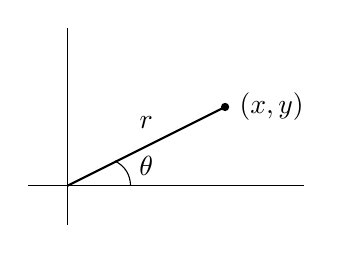
\begin{tikzpicture}
			\draw (-0.5,0) -- (3,0);
			\draw (0,-0.5) -- (0,2);

			\draw[thick] (0,0) -- (2,1);
			\node at (1,1) [below] {$r$};
			\draw (0.8,0) to[bend right] (0.6,0.315);
			\node at (1,0) [above] {$\theta$};
			\node[circle,fill=black,inner sep=0pt,minimum size=3pt,label=right:{$(x,y)$}] at (2,1) {};
		\end{tikzpicture}
	\end{center}

	To convert from Cartesian to polar and back, we use the following formulas
	\[
		x = r\cos\theta \qquad y = r\sin\theta
	\]
	We also adopt the convention that $-\pi \leq \theta \leq \pi$.

	\begin{defi}[Argument]
		We define the \textit{argument} of $z$ to be all $\theta$'s so that $z = r\cos\theta + i r\sin\theta$. We write this as $\arg z$. There is always one value in $(-\pi,\pi]$ and this the \textit{principal value}, written as $\Arg z$. We then have that 
		\[
			\arg z = \{ \Arg z + 2\pi n \, | \, n \in \Z \}
		\]
	\end{defi}

	\begin{eg} $ $
		\begin{enumerate}[label=\alph*.)]
			\item $\Arg(-1) = \pi$, $\arg(-1) = \{ (2n+1)\pi \, | \, n \in \Z \}$.
			\item $\Arg(i) = \pi/2$, $\arg(i) = \{ (2n+\frac{1}{2})\pi \, | \, n \in \Z \}$.
		\end{enumerate}
	\end{eg}

	In Calculus, we have the following Taylor Series
	\begin{align*}
		e^x &= 1 + x + \frac{x^2}{2!} + \frac{x^3}{3!} + \dots \\
		\sin x &= x - \frac{x^3}{3!} + \frac{x^5}{5!} + \dots \\
		\cos x &= 1 - \frac{x^2}{2!} + \frac{x^4}{4!} + \dots
	\end{align*}
	This suggests
	\begin{align*}
		e^{i\theta} &= 1 + i\theta + \frac{i^2\theta^2}{2!} + \frac{i^3\theta^3}{3!} + \frac{i^4\theta^4}{4!} + \dots \\
		&= \left( 1 - \frac{\theta^2}{2!} + \frac{\theta^4}{4!} - \dots \right) + i\left( \theta - \frac{\theta^3}{3!} + \frac{\theta^5}{5!} - \dots \right) \\
		&= \cos\theta + i\sin\theta
	\end{align*}

	Since any $z$ can be written in polar as $z=r\cos\theta + ir\sin\theta$, we can write this as $z=re^{i\theta}$.



\end{document}
